\documentclass{article}

\usepackage{graphicx}
\graphicspath{ {./images/} }

\usepackage{amsmath}

\title{Linjär Algebra}
\author{Pølse}

\begin{document}
\maketitle
\tableofcontents
\pagebreak
\section{Geometriska vektorer}
\textbf{Avsnitt 1.1 och 1.2}
\subsection{}
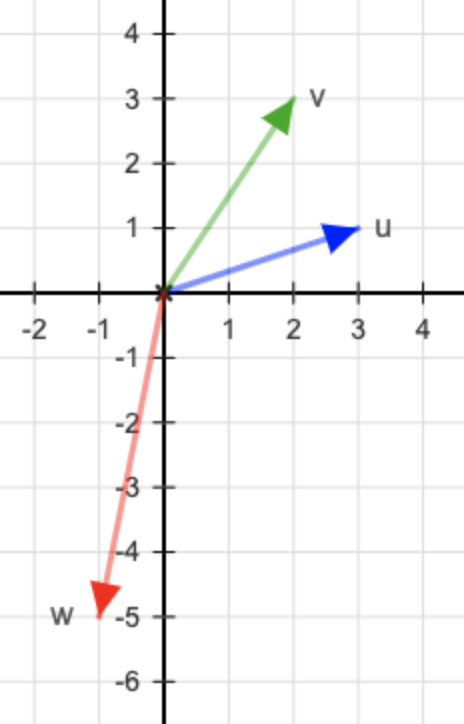
\includegraphics[scale=0.4]{uppg1_1}
\begin{enumerate}
	\item[a)]
	      .\\
	      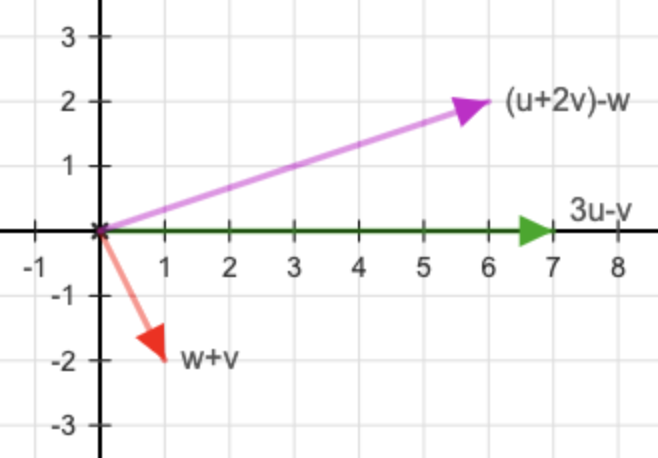
\includegraphics[scale=0.4]{uppg1_1_a}
	\item[b)]
	      .\\
	      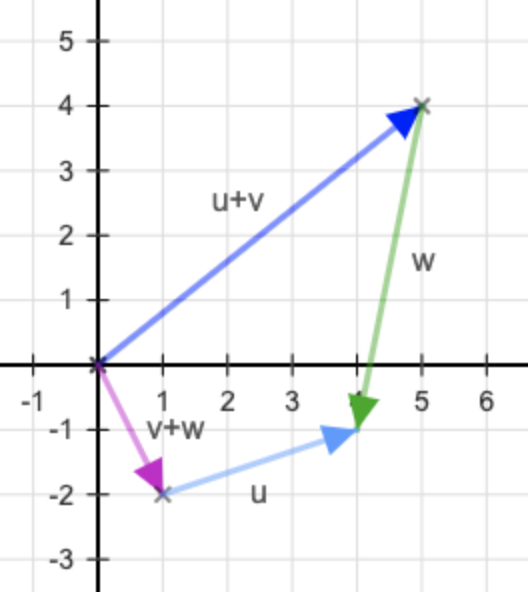
\includegraphics[scale=0.4]{uppg1_1_b}
	\item[c)]
	      \begin{math}
	      	u=
	      	\begin{pmatrix}
	      		3 \\
	      		1 
	      	\end{pmatrix}
	      	,v=
	      	\begin{pmatrix}
	      		2 \\
	      		3 
	      	\end{pmatrix}
	      	,w=
	      	\begin{pmatrix}
	      		-1 \\
	      		-5 
	      	\end{pmatrix}\\
	      	w=su+tv\\
	      	\begin{pmatrix}
	      		-1 \\
	      		-5 
	      	\end{pmatrix}
	      	=s
	      	\begin{pmatrix}
	      		3 \\
	      		1 
	      	\end{pmatrix}
	      	+t
	      	\begin{pmatrix}
	      		2 \\
	      		3 
	      	\end{pmatrix}\\
	      	\begin{cases}
	      		-1=3s+2t \\
	      		-5=s+3t  
	      	\end{cases}\\
	      	(3s+2t)-3(s+3t)=(-1)-3(-5)\\
	      	3s+2t-3s-9t=14\\
	      	-7t=14\\
	      	t=-2\\
	      	s=(-5)-(3t)=(-5)-(-6)=1\\
	      	\begin{cases}
	      		s=1  \\
	      		t=-2 
	      	\end{cases}\\
	      	w=u-2v
	      \end{math}
\end{enumerate}
\subsection{}
\begin{math}
	v\textsubscript{tärna}=
	\begin{pmatrix}
		0   \\
		-40 
	\end{pmatrix}\\
\end{math}
\begin{enumerate}
	\item[a)]
	      \begin{math}
	      	v_\textsubscript{vind}=
	      	\begin{pmatrix}
	      		10 \\
	      		0  
	      	\end{pmatrix},
	      	v\textsubscript{total}=
	      	\begin{pmatrix}
	      		10  \\
	      		-40 
	      	\end{pmatrix}
	      	\\
	      	||v\textsubscript{tärna}||
	      	=\sqrt{v\textsubscript{tärna}\cdot v\textsubscript{tärna}}
	      	=\sqrt{0^2+(-40)^2}
	      	=\sqrt{1600}
	      	=40km/h
	      	\\
	      	||v\textsubscript{total}||
	      	=\sqrt{v\textsubscript{total}\cdot v\textsubscript{total}}
	      	=\sqrt{10^2+(-40)^2}
	      	=\sqrt{100+1600}
	      	=\sqrt{1700}
	      	=10\sqrt{17}
	      	\approx 41.23km/h
	      	\\
	      	\cos(\theta)
	      	=\frac{v\textsubscript{tärna}\cdot v\textsubscript{total}}{||v\textsubscript{tärna}||*||v\textsubscript{total}||}
	      	=\frac{0*10+(-40)*(-40)}{40*10\sqrt{17}}
	      	=\frac{1600}{40*10\sqrt{17}}
	      	=\frac{4}{\sqrt{17}}
	      	\\
	      	\theta=
	      	\cos^{-1}(\frac{4}{\sqrt{17}})
	      	\approx 14.04^{\circ}
	      \end{math}
	\item[b)]
	      \begin{math}
	      	||v_\textsubscript{vind}||=10\\
	      	v_\textsubscript{vind}=
	      	\begin{pmatrix}
	      		\sqrt{50} \\
	      		\sqrt{50} 
	      	\end{pmatrix},
	      	v\textsubscript{total}=
	      	\begin{pmatrix}
	      		\sqrt{50}    \\
	      		\sqrt{50}-40 
	      	\end{pmatrix}
	      	\\
	      	||v\textsubscript{tärna}||
	      	=\sqrt{v\textsubscript{tärna}\cdot v\textsubscript{tärna}}
	      	=\sqrt{0^2+(-40)^2}
	      	=\sqrt{1600}
	      	=40km/h
	      	\\
	      	||v\textsubscript{total}||
	      	=\sqrt{v\textsubscript{total}\cdot v\textsubscript{total}}
	      	=\sqrt{\sqrt{50}^2+(\sqrt{50}-40)^2}
	      	=\sqrt{50+(50-80\sqrt{50}+1600)}
	      	=\sqrt{1700-80\sqrt{50}}
	      	=\sqrt{1700-400\sqrt{2}}
	      	=10\sqrt{17-4\sqrt{2}}
	      	\approx 33.68km/h
	      	\\
	      	\cos(\theta)
	      	=\frac{v\textsubscript{tärna}\cdot v\textsubscript{total}}{||v\textsubscript{tärna}||*||v\textsubscript{total}||}
	      	=\frac{0*\sqrt{50}+(-40)*(\sqrt{50}-40)}{400\sqrt{17-4\sqrt{2}}}
	      	=\frac{1600-40\sqrt{50}}{400\sqrt{17-4\sqrt{2}}}
	      	=\frac{1600-200\sqrt{2}}{400\sqrt{17-4\sqrt{2}}}
	      	=\frac{8-\sqrt{2}}{2\sqrt{17-4\sqrt{2}}}
	      	\\
	      	\theta
	      	=\cos^{-1}(\frac{8-\sqrt{2}}{2\sqrt{17-4\sqrt{2}}})
	      	\approx 12.12^{\circ}
	      \end{math}
	\item[c)]
	      \begin{math}
	      	v_\textsubscript{vind}=
	      	\begin{pmatrix}
	      		10 \\
	      		0  
	      	\end{pmatrix},
	      	v\textsubscript{total}=
	      	\begin{pmatrix}
	      		0 \\
	      		x 
	      	\end{pmatrix},
	      	v\textsubscript{tärna}=
	      	\begin{pmatrix}
	      		-10 \\
	      		x   
	      	\end{pmatrix}
	      	\\
	      	||v\textsubscript{tärna}||=40
	      	\\
	      	x=
	      	\sqrt{40^2-(-10)^2}
	      	=\sqrt{1600-100}
	      	=\sqrt{1500}
	      	=10\sqrt{15}
	      	\\
	      	||v\textsubscript{total}||
	      	=10\sqrt{15}
	      	\approx 38.73km/h
	      	\\
	      	\cos(\theta)
	      	=\frac{v\textsubscript{tärna}\cdot v\textsubscript{total}}{||v\textsubscript{tärna}||*||v\textsubscript{total}||}
	      	=\frac{0*(-10)+(10\sqrt{15})^2}{40*10\sqrt{15}}
	      	=\frac{(10\sqrt{15})^2}{40*10\sqrt{15}}
	      	=\frac{10\sqrt{15}}{40}
	      	=\frac{\sqrt{15}}{4}
	      	\\
	      	\theta
	      	=\cos^{-1}(\frac{\sqrt{15}}{4})
	      	\approx 14.48^{\circ}
	      \end{math}
\end{enumerate}
\subsection{}
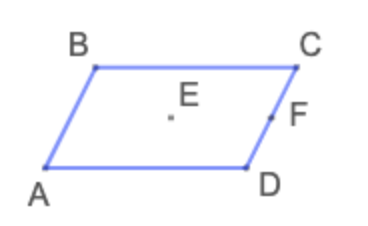
\includegraphics[scale=0.6]{uppg1_3}
\begin{enumerate}
    \item[a)]
        \begin{math}
            E
            =\frac{1}{2}\vec{AC}
            =\frac{1}{2}(\vec{AB}+\vec{AD})
            =\frac{1}{2}\vec{AB}+\frac{1}{2}\vec{AD}
        \end{math}
    \item[b)]
        \begin{math}
            \vec{AB}
            =\frac{1}{2}\vec{AC}-\frac{1}{2}\vec{BD}
            \\
            \vec{AD}
            =\frac{1}{2}\vec{AC}+\frac{1}{2}\vec{BD}
        \end{math}
    \item[b)]
        \begin{math}
            \vec{AF}
            =\vec{AD}+\frac{1}{2}\vec{AB}
            =(\frac{1}{2}\vec{AC}+\frac{1}{2}\vec{BD})+\frac{1}{2}(\frac{1}{2}\vec{AC}-\frac{1}{2}\vec{BD})
            =\frac{1}{2}\vec{AC}+\frac{1}{2}\vec{BD}+\frac{1}{4}\vec{AC}-\frac{1}{4}\vec{BD}
            =\frac{3}{4}\vec{AC}+\frac{1}{4}\vec{BD}
        \end{math}
\end{enumerate}
\textbf{Avsnitt 1.3}
\subsection{}
\begin{math}
    ||u||=1, 
    ||v||=1,
    \theta=\pi/3
\end{math}
\begin{enumerate}
    \item[a)]
        \begin{math}
            u\cdot v
            =||u||*||v||*\cos(\theta)
            =1*1*\cos(\pi/3)
            =\cos(\pi/3)
            =\frac{1}{2}
        \end{math}
    \item[b)]
        \begin{math}
            (3u-4v)\cdot (u+5v)
            =3u\cdot u+3u\cdot 5v+(-4)v\cdot u+(-4)v\cdot 5v
            =3(u\cdot u)+15(u\cdot v)-4(v\cdot u)-20(v\cdot v)
            =3*1+15*0.5-4*0.5-20*1
            =3+7.5-2-20
            =\frac{6}{2}+\frac{15}{2}-\frac{4}{2}-\frac{40}{2}
            =\frac{-23}{2}
        \end{math}
    \item[c)]
        \begin{math}
            ||3u+4v||
        \end{math}
\end{enumerate}
\section{Matriser}
\section{Geometriska linjära avbildningar}
\section{Rummet $R^n$}
\section{Linjära ekvationssytem}
\section{Determinant}
\section{Baser}
\section{Egenvärden och vektorer}
\section{Grafer och grannmatriser}
\end{document}

\subsection{}
\begin{math}
	
\end{math}